\section{Datathons}

% Description of datahton
A datathon is an event similar to a hackathon where people come together over a certain time period, commonly 24 hours to work on problems with a specific dataset. There are a number of steps involved in a datathon including preparing, planning, recruiting participants, arranging an appropriate venue, preparing the data for exploration, logistics, and hosting the event. We describe the benefits of datathons and outline our experience at running four datathons.

\subsection{Benefits}

Datathons provide unique opportunities for computer science students to acquire experience in working with data, participating in interdisciplinary teams, and gain project management skills.
\begin{itemize}
\item Data skills.  Data and analytics are important throughout computer science, whether in working directly with data, handling the data associated with software development such as testing results, as well as in communicating data to others
\item Interdisciplinary teams.  Many areas of computer science practice rely on working with non-computer scientists.  The most prevalent example is that of requirements gathering with clients for development projects.   However many other areas such as in game development, tools development for scientists, visualization design, etc.
\item	Project management skills. Blah, blah, blah
\end{itemize}


\section{Case Studies}

In our case studies we will discuss two types of datathons.  The first is a slight variation on a hackathon where the goal is to form teams and then create an app that builds on public datasets.  The second is a more data-focused approach where participants work with organization’s dataset, providing expertise in working with data that the organization lacks and helping the organization answer questions that they lack the resources to answer themselves.

%------------------------------------------------------------
%         CODE
%------------------------------------------------------------
\subsection{Canadian Open Data Experience}

Data-focused hackathons are a popular means that local, regional, and federal governments are actively sponsoring to gather interest in open government data initiatives.  These events aim to create apps that make use of recently released datasets; generating interest among developers and technology innovators into government datasets as well as with hope of creating useful and popular applications that will draw public interest and attention to these datasets.

Our involvement has been with the Government of Canada's Canadian Open Data Experience (CODE)\footnote{https://www.canadianopendataexperience.ca/}.  This event encourages developers to create applications using the government's open data portal.  While self-organized teams were free to explore the data ahead of the event; the event itself consisted of a 48-hour coding sprint in which three broad areas of application themes were announced, and the apps were developed.  After the event a shortlist of 15 finalist teams from across the country was created and then the prize winners were selected: one for each application theme, a ``fan favourite'', and a best student team.  We organized two hubs as part of the CODE competition in 2014 and 2015.

%The Canadian Open Data Experience (CODE)\footnote{https://www.canadianopendataexperience.ca/} is an intense 48-hour coding sprint where innovators from coast to coast compete to build the best app utilizing federal government data from Canada's Open Government portal. We organized two hubs as part of the CODE competition in 2014 and 2015. 

In 2014 four teams participated with four members per team.  One team made the grand final of the top 15 teams and presented their app in front of judges in Toronto.  In 2015 fourteen participants split into five teams.  

\begin{figure*}[!htb] % this puts images exactly where you want them
\begin{center}
\subfigure[CODE 2014 - Brainstorming Session.]{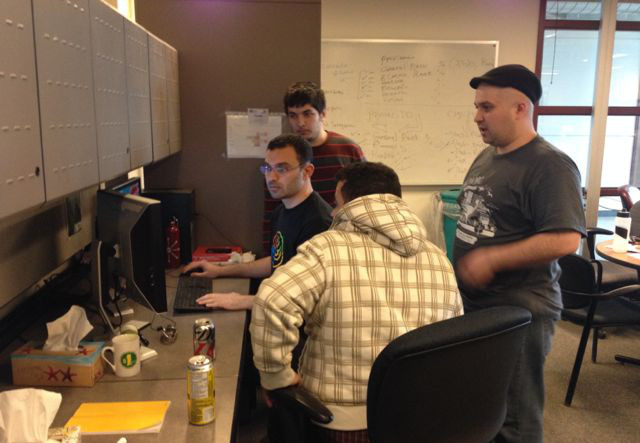
\includegraphics[keepaspectratio,width=8cm]{images/code-2014-brainstorm.jpg}\label{fig:brainstorm}}
\subfigure[Data For Good 2014 - Introductory Session.]{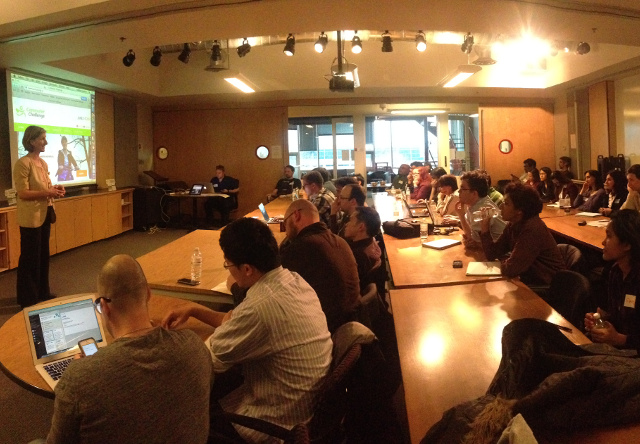
\includegraphics[keepaspectratio,width=8cm]{images/dfg-2014-introductory.jpg}\label{fig:sdv}}
\caption{Datathons Case Study - illustrating different aspects of the datathons.}
\label{fig:datathons}
\end{center}
\end{figure*}

%------------------------------------------------------------
%         DFG
%------------------------------------------------------------
\subsection{Data For Good}

Data for Good (DFG)\footnote{http://www.meetup.com/Data-for-Good-Calgary/} is a community organization inspired by DataKind.org and is working for positive social action through ``data in the service of humanity". Data for Good in Calgary brings together data scientists with social organizations through a  collaborative approach that leads to shared insights, greater understanding, and positive action of data. Data for Good leads a community of data scientists from the community and university to inspire a new way of using the skills and tools of corporations \& governments, to meet the needs of the NFP/NGO and social innovation sector.

The DFG datathon followed much less of the hackathon prototype.  Rather than creating a specific application, the goal instead was to help a social good organization make use of their data.  Among non-profits this scenario of having large amounts data but lacking the resources to make use of it is quite common.  Non-profits gather a great deal of data to support grant applications, reporting requirements, and in tracking operations.  However, typical non-profit funding usually includes very little or no funding for administrative overhead, such as data management and analysis.  Consequently these organizations make minimal use of this data but are often keen to see the data used to improve their efforts and organization.  
Naturally this is much less of a self-contained event, requiring a great deal of collaboration with the organization, preparation of their datasets, and in creating reasonably scoped objectives that can be accomplished by the group over the course of the weekend.


DFG organizes regular meetups for it's members and hosts weekend datathon events. A DataThon is a weekend event that matches up selected social organizations (that have well-defined data problems) with a team of volunteer data scientists to tackle their data-related challenges over a 24-48 hous period. The participants are fed throughout the weekend event \& the results are presented to the social organizations at the end of the event. Some may refer to these types of events as "Hack-a-Thons", etc. These events are completely free for the participants and serve to energize, educate, and provide direct benefit to the NFP/NGO organizations, as well as to enlighten social sector groups about the power of being data-driven.


Suatainable Alberta Association\footnote{http://www.meetup.com/Data-for-Good-Calgary/events/175671942/}

Distree Centre\footnote{http://www.meetup.com/Data-for-Good-Calgary/events/221869098/}


